\documentclass[acmtog]{acmart}
\usepackage{listings}
% Title portion
\title{Assignment 1 : Creating a simple keyframe-based animation} 
\author{Name:\quad Tianyuan Wu \\ student number:\quad 63305667
	\\email:\quad wuty@shanghaitech.edu.cn}

% Document starts
\begin{document}
\maketitle

\vspace*{2 ex}


\section{Introduction}
In this assignment, I implemented an simple keyframe-based animation using cubic spline interpolation. 
In implementation, I set 4 key frames to indentify 4 different poses of the model, then use cubic 
spline interpolation to generate a smooth animation. In this assignment, not only a smooth, window-based 
animation has been generated, the velocity control of the object is also implemented (we can control 
the velocity of the object by command-line arguments). What's more, the Eular angle of the model can be 
logged dynamically, and a visualization script is also implemented. The program is based on \texttt{OpenGL}, 
\texttt{TinyObjLoader}, and \texttt{Eigen}, has been compiled with \texttt{Apple clang 12.0.0} and 
tested on \texttt{macOS 10.15}.

\section{Implementation Details}
\subsection{Keyframe Selection}
In this assignment, we use Eular angles (In this section, an Eular angle is represented as a t
riple $(\alpha, \beta, \gamma)$.) to represent the pose of the model. \\
To generate a smooth animation, 4 key frames are set to represent different poses of the model:
\begin{table}[h]
	\begin{tabular}{|c|c|c|c|}
		\hline
		 & $\alpha$ & $\beta$ & $\gamma$\\
		\hline
		Keyframe1 & 3.141593 & 0 & 0\\
		\hline
		Keyframe2 & 3.141593 & 1.0472 & 0.5236\\
		\hline
		Keyframe3 & 3.141593 & 0 & 0\\
		\hline
		Keyframe4 & 3.141593 & -1.0472 & -0.5236\\
		\hline
	\end{tabular}
\end{table}
The reason of such a selection is, Keyframe1 and Keyframe3 represent the original pose of the model, 
Keyframe2 represents the left-side pose, and Keyframe4 represents the right-side pose (shown in Fig.1-3).\\
Then, we repeat this 4 keyframes ($f_1, f_2, f_3, f_4$) to generate a keyframe sequence, like 
$f_1, f_2, f_3, f_4, f_1, f_2, \ldots$. 
\begin{figure}[h]
	\begin{center}
		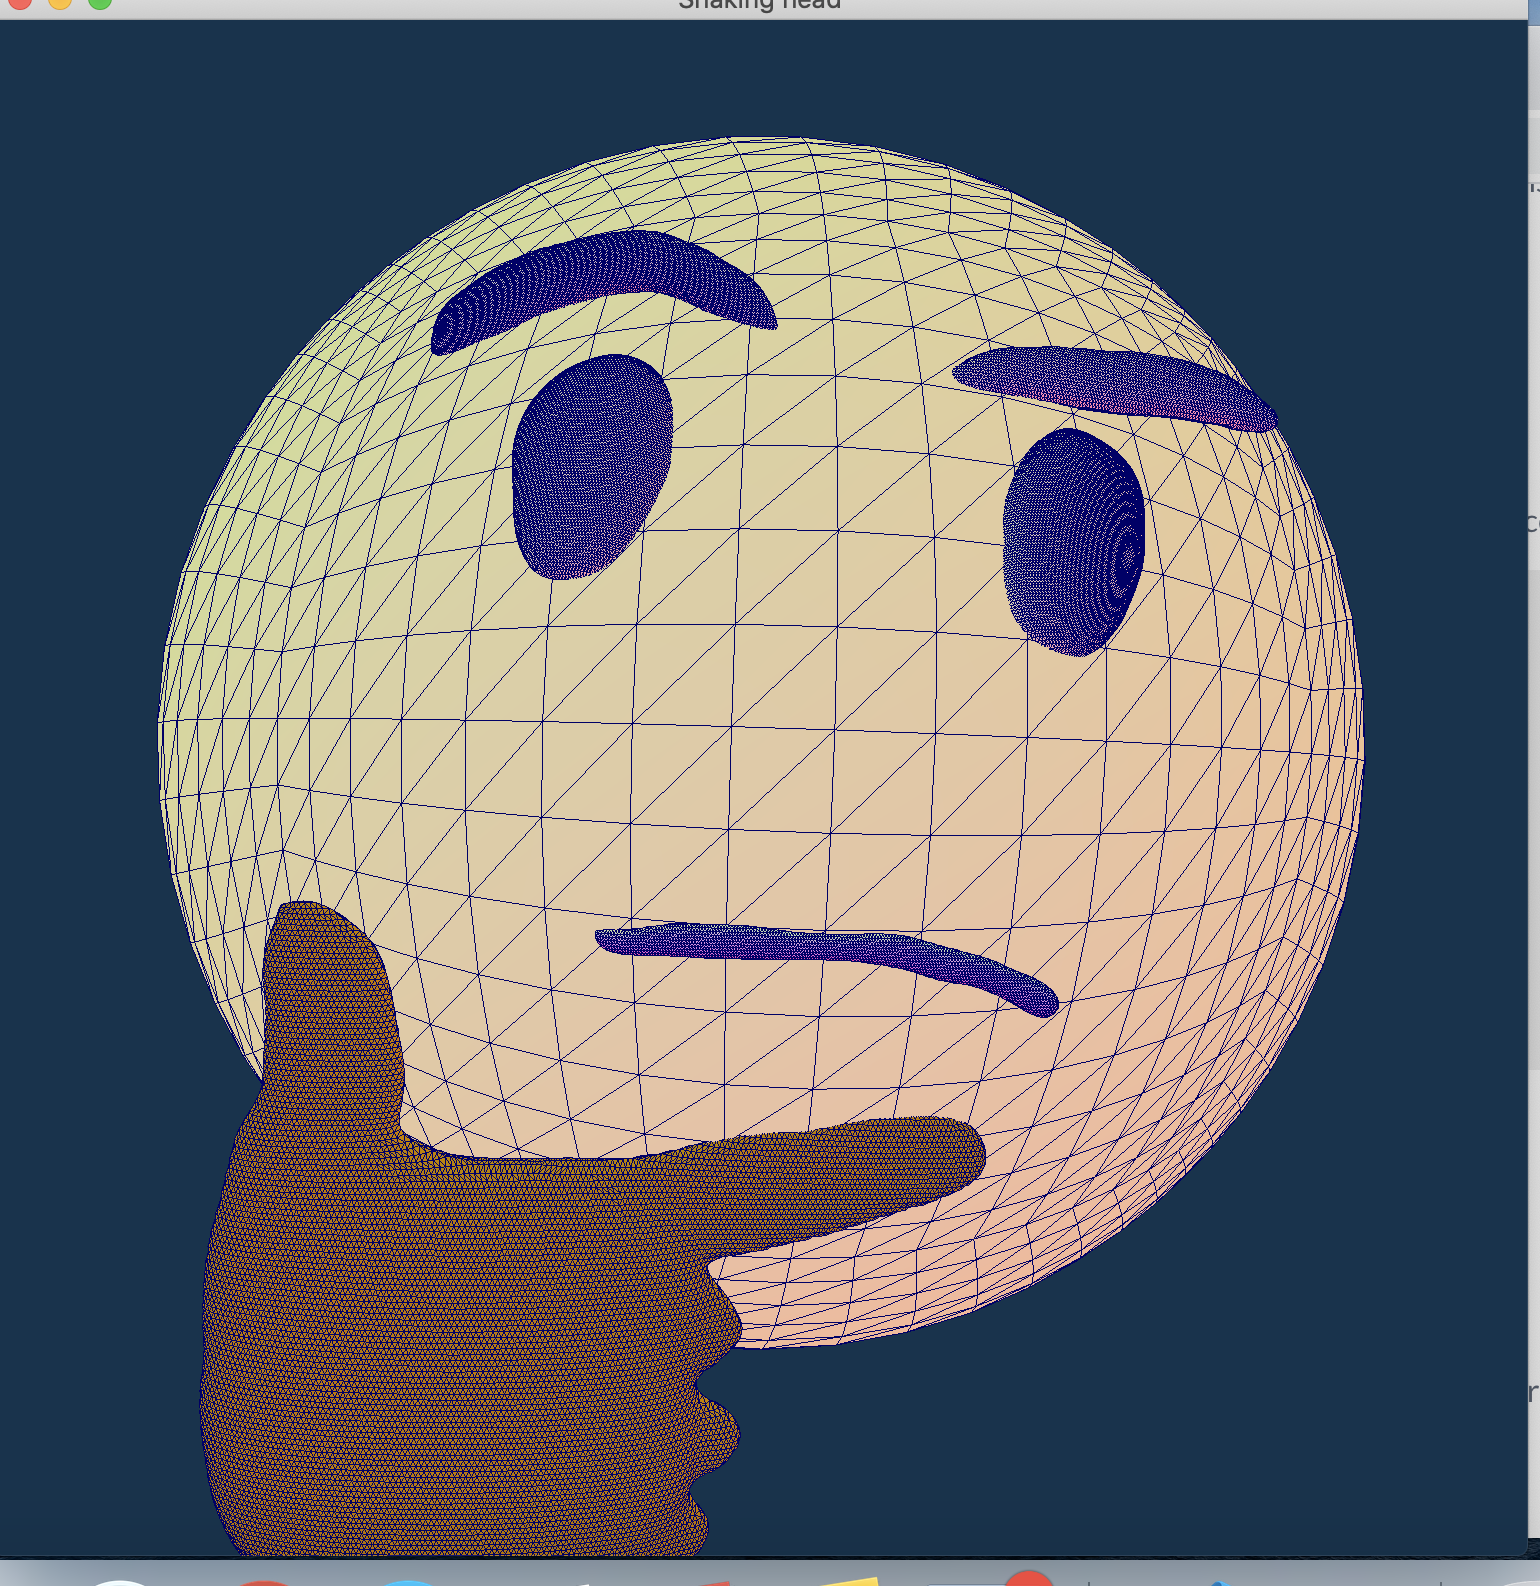
\includegraphics[scale=0.17]{origin.png}
	\end{center}
	\caption{Original pose of the model}
\end{figure}
\begin{figure}[h]
	\begin{center}
		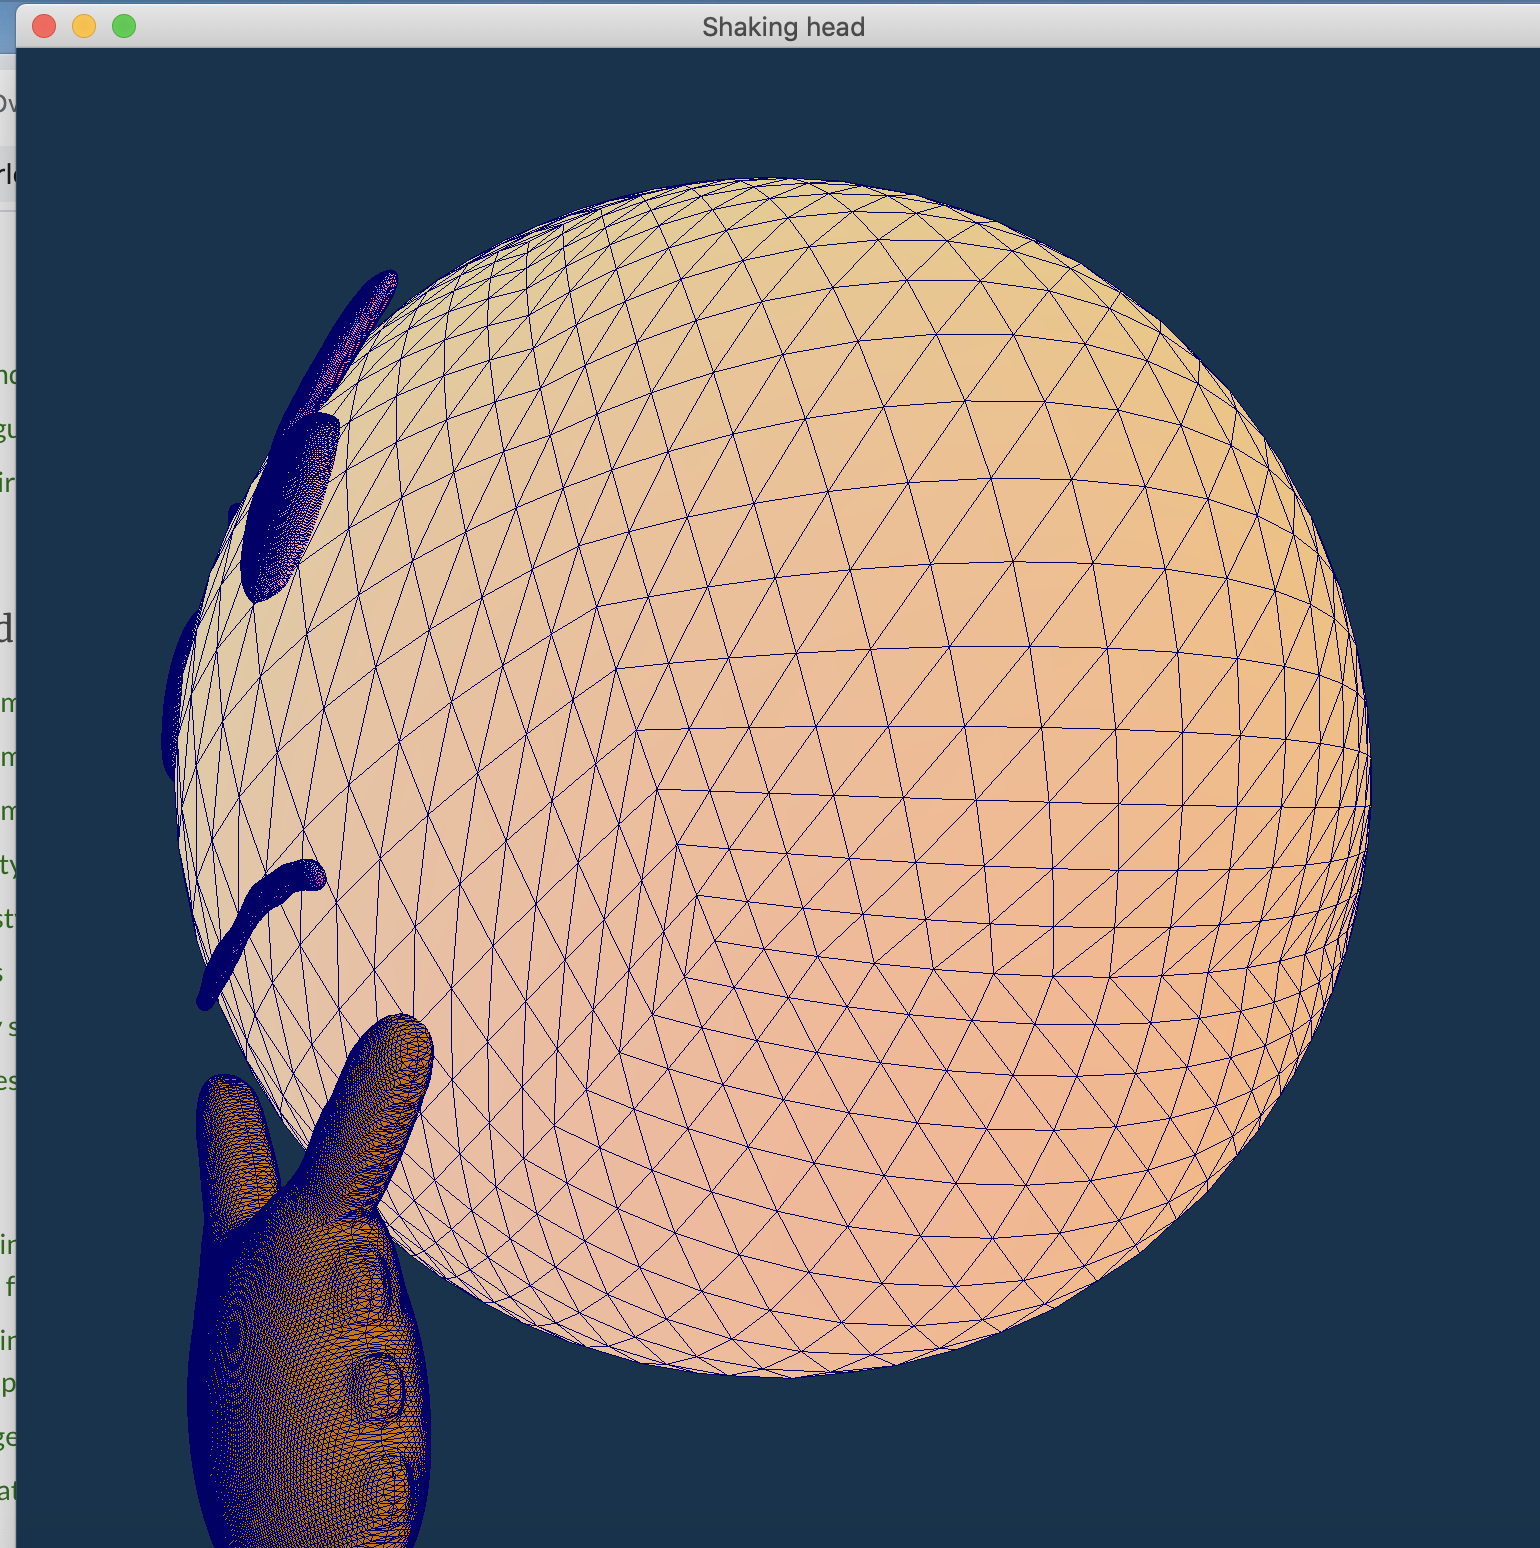
\includegraphics[scale=0.17]{left.png}
	\end{center}
	\caption{Left-side pose of the model}
\end{figure}
\begin{figure}[h]
	\begin{center}
		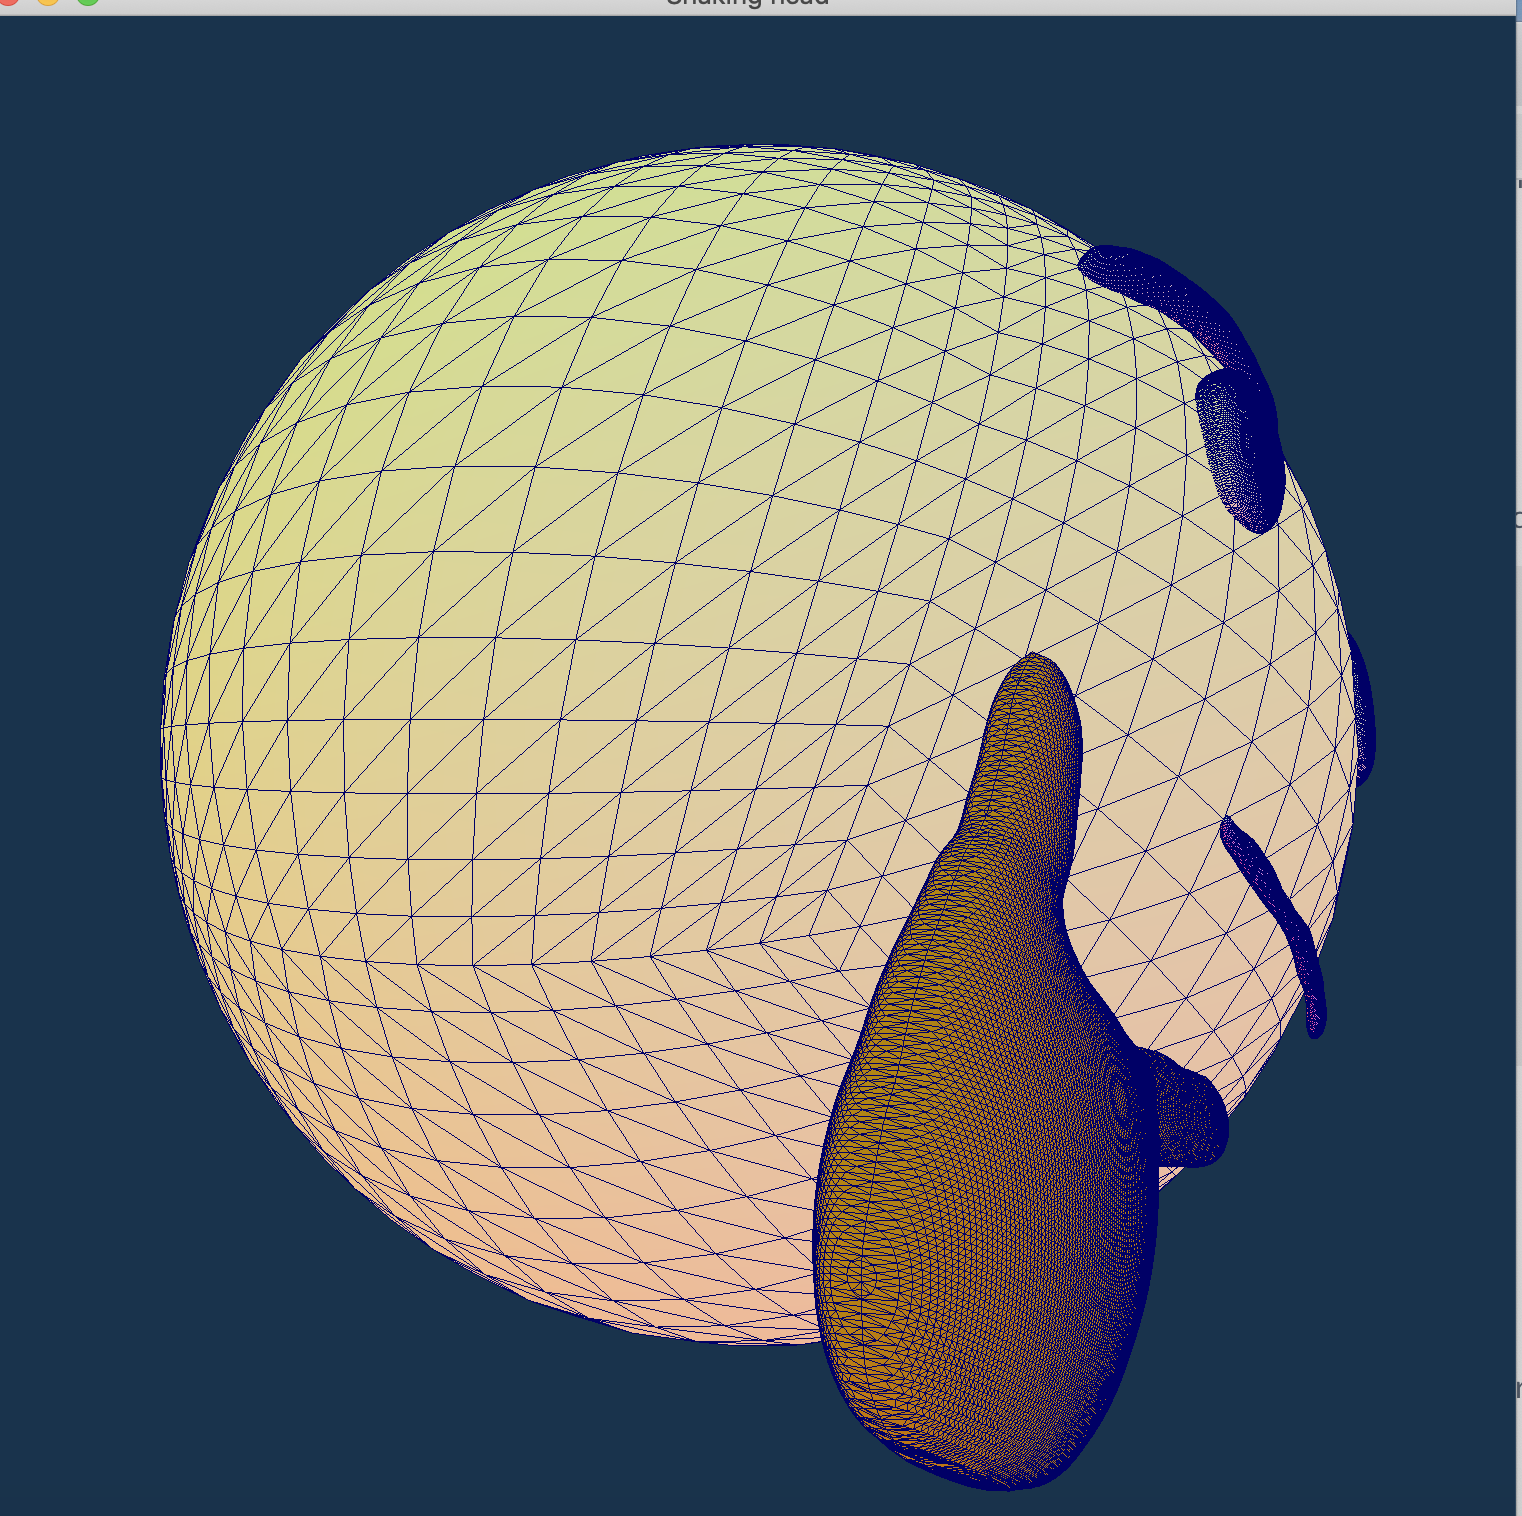
\includegraphics[scale=0.17]{right.png}
	\end{center}
	\caption{Right-side pose of the model}
\end{figure}
These keyframes are hard-coded in \texttt{viewer.cpp} now, and user can create/modify key frames 
by modifying the keyframe array and re-compile the code.

\newpage
\vspace*{2 ex}
\subsection{Algorithm}
In this assignment, I use \textbf{cubic spline interpolation} to generate frames 
between keyframes.\\
Suppose the the keyframe sequence is $(\alpha_1, \beta_1, \gamma_1), (\alpha_2, \beta_2, \gamma_2), \ldots$. 
For some specific dimension (e.g. $\alpha$), the interpolation process are described below.\\
We have $n+1$ keyframes $\alpha_0, \alpha_1, \ldots, \alpha_{n}$, and we need $n$ cubic functions $S_1(x), S_2(x), \ldots, S_n(x)$, 
which satisfies
$$
\begin{cases}
	S_i(x_i) = \alpha_i\\
	S_i'(x_{i+1}) = S_{i+1}'(x_{i+1})\\
	S_i''(x_{i+1}) = S_{i+1}''(x_{i+1})
\end{cases}
$$
Let
$$S_i(x) = a_i + b_i(x-x_i) + c_i(x-x_i)^2 + d_i(x-x_i)^3$$
the step:
$$h_i = x_{i+1} - x_i$$
and let
$$m_i = S''_{i}(x_i) = 2c_i$$
By the constraints shown above, we have
$$
\begin{cases}
	a_i = \alpha_i\\
	b_i = \frac{\alpha_{i+1} - \alpha_i}{h_i} - \frac{h_im_i}{2} - \frac{h_i(m_{i+1} - m_{i})}{6}\\
	c_i = \frac{m_i}{2}\\
	d_i = \frac{m_{i+1} - m_{i}}{6h_i}
\end{cases}
$$
and $m_i$ can be solved by the following equation (use natural spline):
$$
\begin{bmatrix}
	1 & 0 & 0 & \ldots & 0\\
	h_0 & 2(h_0 - h_1) & h_1 & \ldots & 0\\
	& &\ldots & &\\
	\ldots & 0 & h_{n-2} & 2(h_{n-2} - h_{n-1}) & h_{n-1}\\
	0 & \ldots & 0 & 0 & 1
\end{bmatrix}
\begin{bmatrix}
	m_0\\
	m_1\\
	\ldots\\
	m_n
\end{bmatrix} = 
\begin{bmatrix}
	0\\
	y_0\\
	\ldots\\
	y_{n-2}\\
	0
\end{bmatrix}
$$
where $y_i = \frac{\alpha_{i+2} - \alpha_{i+1}}{h_{i+1}} - \frac{\alpha_{i+1} - \alpha_{i}}{h_{i}}$\\
By similar ways, we can get the interpolations of $\beta$ and $\gamma$, and generate internal frames.

\subsection{Code Implementation}
In this assignment, I use \texttt{TinyObjLoader} to load the mesh at first, then use a OpenGL based 
shader to render the mesh (based on the \texttt{examples/viewer} in \texttt{TinyObjLoader}). To generate 
the animation, I implemented a solver to do the interpolation and calculate the next Eular angle. Then 
we need to convert the Eular angle to a quaternion (implemented in \texttt{helpers.cpp}) and build a 
rotation matrix. Finally, we render the mesh and watch it from the calculated position.\\
The code has been compiled under macOS 10.15, with Apple clang 12.0.0, and the performance of this implementation 
can reach about 60 frames per second on CPU.\\
Prerequisites: \texttt{GLEW, GLFW, GLTools, Eigen3}\\
Third party libraries used: \texttt{TinyObjLoader}

\section{Results}
In this implementation, a smooth animation is generated when run the program. A capture of the animation is 
shown is Fig.4\\
\begin{figure}[H]
	\begin{center}
		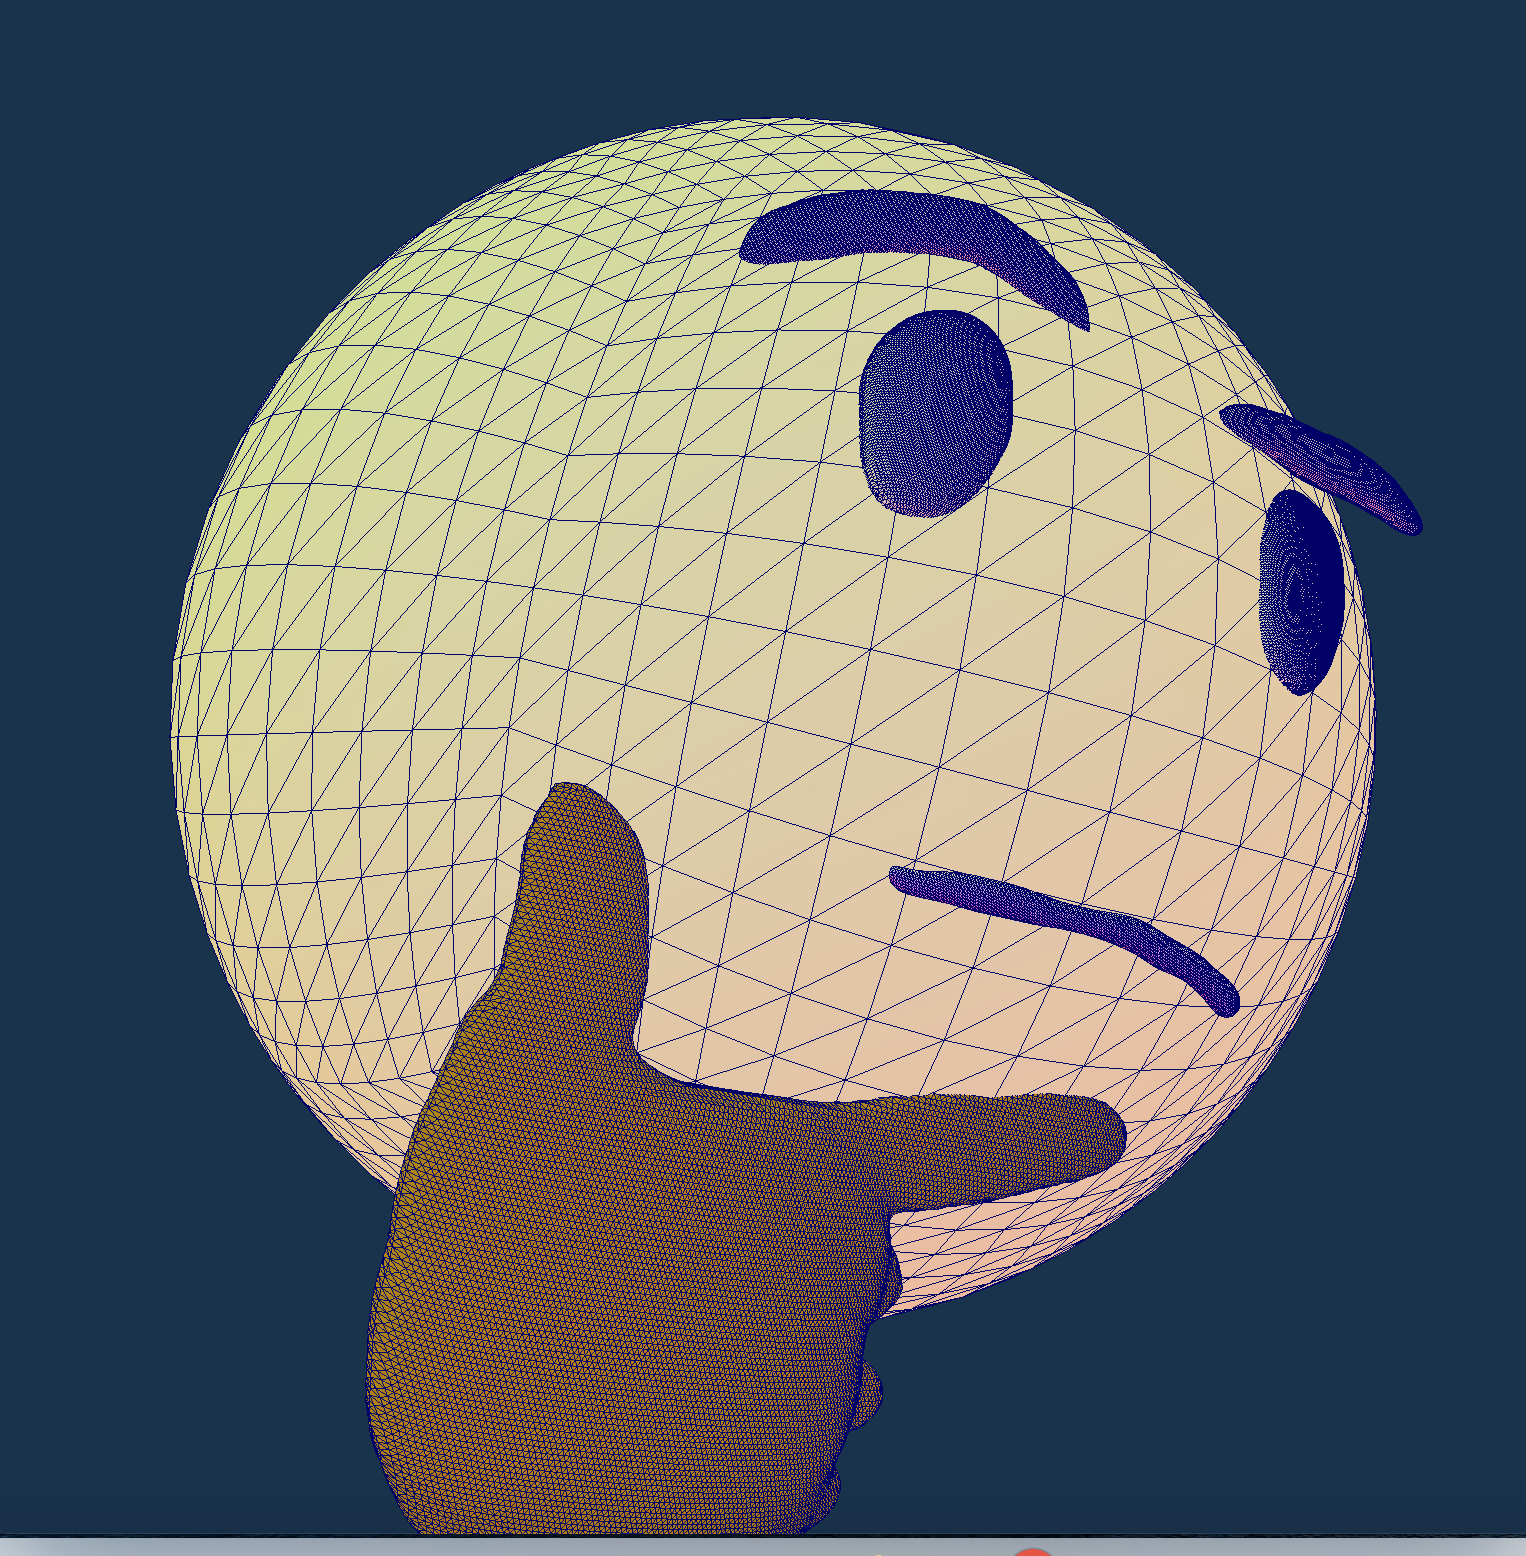
\includegraphics[scale=0.17]{frame.png}
	\end{center}
	\caption{A capture of the animation}
\end{figure}
Also, the change of Eular angle has been logged, Fig.5 shows the dynamic change of Eular angle by time.\\
\begin{figure}[H]
	\begin{center}
		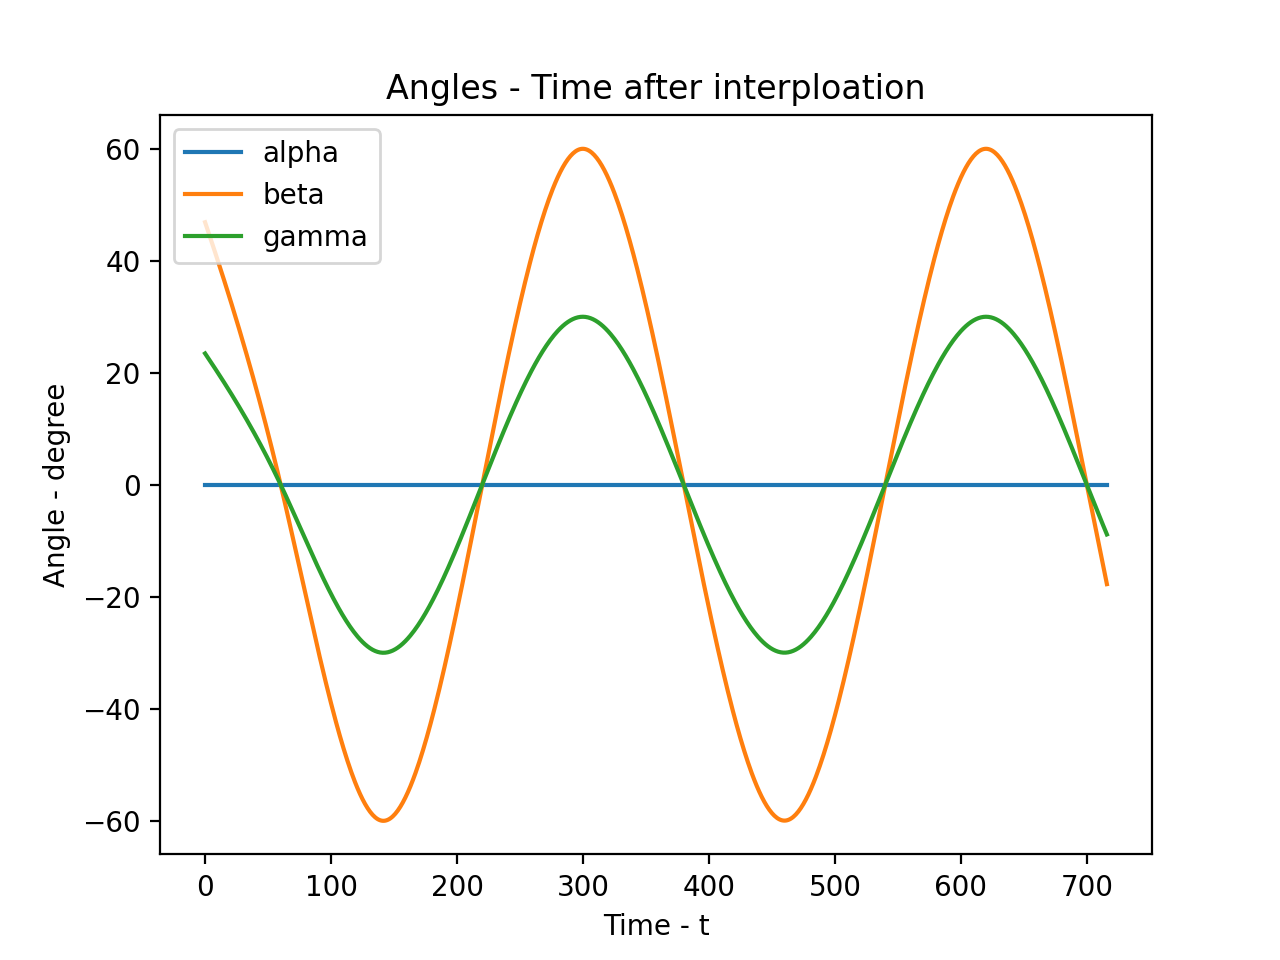
\includegraphics[scale=0.5]{angles.png}
	\end{center}
	\caption{Eular angle - time diagram}
\end{figure}
The velocity of the model can be adjusted using command line options. For example, if you want to add 
80 frames between 2 key frames, you can type \texttt{./shake\_head 80} in command line to run the program. 
When no additional command line options are given, the number of interploated frames between 2 key frames 
are set to 50 by default.\\
This implementation also has a relative high performance, which can reach about 60 frames per second on CPU
(the FPS statistics are are logged in the console for every second). 

\end{document}
